\frame{
\frametitle{Why Topological Data Analysis?}
\framesubtitle{``Data has shape and the shape matters.'' - Gunnar Carlsson}
\begin{block}{}
 Today, Data is high-dimensional, \onslide<2->{HUGE,}
 \onslide<3->{present everywhere}
 \vspace{.2in}
 \begin{columns}
  \column{.32\textwidth}
 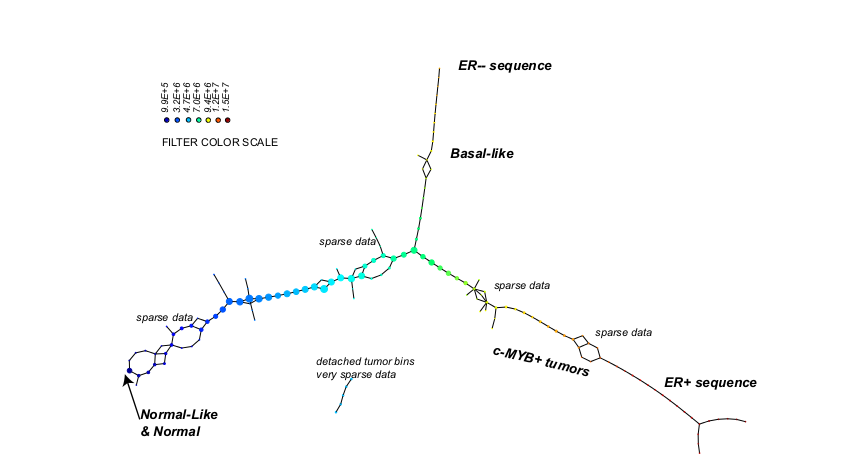
\includegraphics[width=\textwidth,height=1.25in]{examples/stanford-reeb}%
   \\
   ---------------------\\
   \scriptsize{Nicolaua, Levine, and Carlsson, PNAS 2011}
   \column{.32\textwidth}
   \onslide<2->{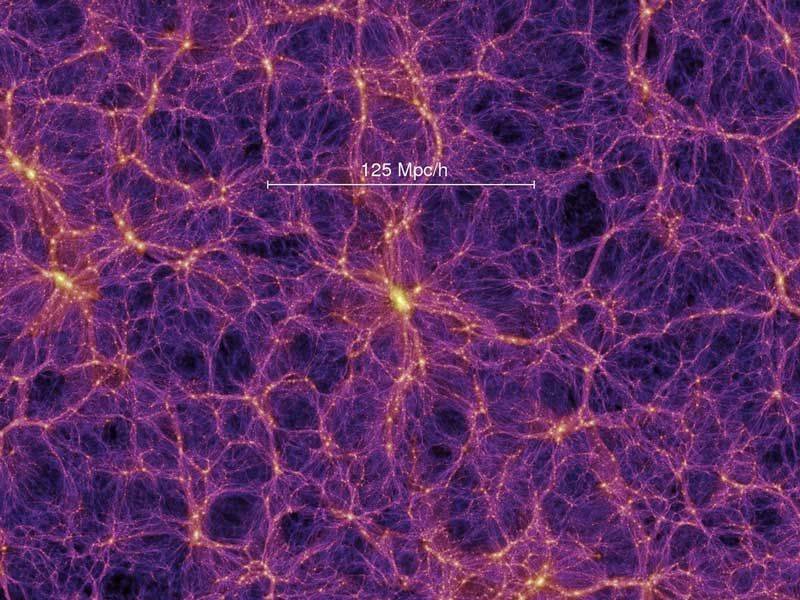
\includegraphics[width=\textwidth]{examples/cosmic-web}
   \\
   ---------------------\\
   \scriptsize{http://astrobites.com/}
   }%
   \column{.32\textwidth}
   \onslide<3->{
   \vspace{.2in} \\
   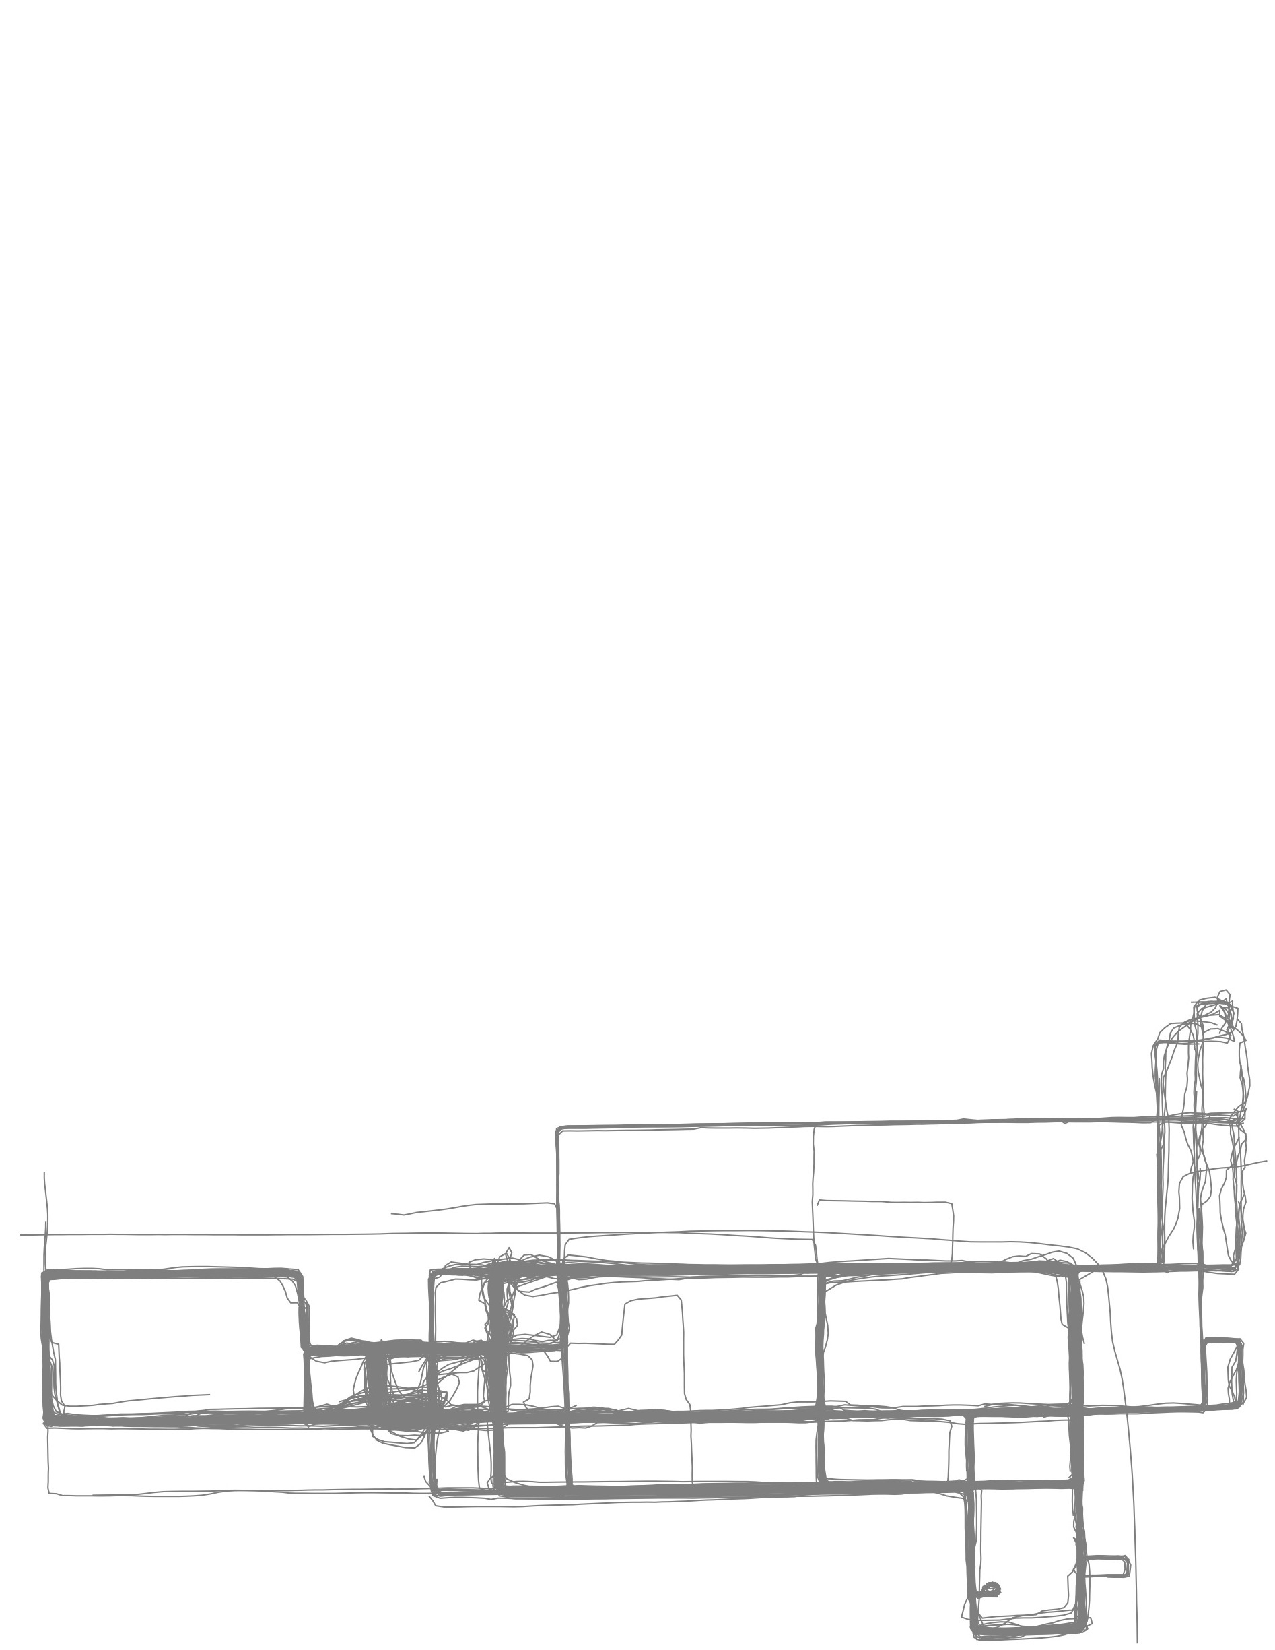
\includegraphics[width=\textwidth]{examples/chicago-tracks}
   \vspace{.2in} \\
   ---------------------\\
   \scriptsize{\url{www.mapconstruction.org}}
   }
 \end{columns}
 \vspace{.2in}
 ... and needs to be summarized, analyzed, and compared!

\end{block}
}

\frame{
    \todo{revise these questions perhaps}
    \begin{columns}
        \column{.45\textwidth}
        \begin{block}{Summarize and Analyze}
            \begin{itemize}
                \item What is this shape?
                \item How many components / populations?
                \item Can we categorize? (Classification)
                \item What are the parameters? (Inference)
                \item Does the descriptor provide stable information?
            \end{itemize}
        \end{block}

        \pause
        \column{.45\textwidth}
        \begin{block}{Compare}
            \begin{itemize}
                \item Are these the same (in distribution)?
                \item Has something changed?
                \item Where is the change?
                \item Which is bigger?
                \item What is the relationship between $X$ and $Y$? (Regression)
            \end{itemize}
        \end{block}
    \end{columns}
}

\frame{
    \frametitle{Most Important Questions}

    \pause
    \begin{block}{}
        1. Which Descriptor best captures our data?
    \end{block}

    \pause
    \begin{block}{}
        2. How do we measure distance between descriptors?
    \end{block}
}
